\chapter{Heurístico}
El algoritmo heurístico que se ha creado para el problema está inspirado en el metahurístico \textit{GRASP (Greedy Randomized Adaptive Search Procedure)}, sobre el que se han realizado una serie de modificaciones para adaptarlo al modelo en cuestión. A continuación se explicará el funcionamiento de un GRASP, para después explicar el algoritmo propuesto comparando sus diferencias y semajanzas.

\section{GRASP}
Un Grasp es un metaheurístico constructivo desarrollado inicialmente por T. Feo   M. Resende, y se definie como \textcolor{red}{->cita libro Abraham<-} \textit{un GRASP es un procedimiento multiarranque en el que cada arranque se corresponde con una iteración. Cada iteracción tiene dos fases bien diferenciadas, la fase de construcción, que se encarga de obtener una solución factible de alta calidad; la fase de mejora, que se basa en la optimización (local) de la solución obtenida en la primera fase.}

\subsection{Fase constructiva}
La fase constructiva es un proceso iterativo en el que se construye una solución elemento a elemento.\\
Inicialmente se parte de un componente o conjunto de componentes que conforman una solución parcial, y no serán seleccionables. Posteriormente se ordenan los elementos seleccionables utilizando una función voraz (Greedy), la cual asignará a cada elemento un valor que indique como variaría la función objetivo si se añade a la solución parcial.\\
Una vez están ordenados todos los elementos seleccionables, hay que seleccionar qué elemento es añadido a la solución parcial. GRASP no añade el mejor candidato posible, ya que esto no garantiza que se obtenga la solución óptima, sino que se elije aleatoriamente un candidato del conjunto de candidatos restringido (o RCL por sus siglas en inglés). Para crear esta RCl, se crea un conjunto de candidatos que cumplan
\begin{equation}\\
{RCL}_{umbral} = (c_{min}+\alpha(c_{max} - c_{min} ))
\end{equation}
donde $c_{min}$ y $c_{max}$ son respectivamente los valores más bajo y más alto del coste asignado a los elementos seleccionables, y el parámetro  :$\alpha : 0\leq \alpha \leq1$ determina el umbral permitido, de forma que se escoge un candidato aleatorio. Si fijamos $\alpha=1$, en la RCL solo contaríamos con el mejor candidato, y sería una función miope pura. Por el contrario si fijamos $\alpha=0$, serán seleccionados todos los candidatos.\\

Una vez seleccionado el elemento o elementos, se introducen en la solución parcial y se les marca como no seleccionables. El resto de candidatos siguen siendo seleccionables, por tanto cuando se les vuelva a evaluar para ser candidatos, sus valores serán distintos a los de la iteración anterior, ya que la solución parcial ha variado al haber añadido el último elemento conjunto de candidatos.\\

La fase constructiva finaliza cuando se dispone de una solución factible.
\subsection{Fase de mejora}
Pero la fase constructiva no garantiza que la solución sea óptima respecto a su vecindad. Por ello GRASP incorpora la fase de mejora, que consiste en un procedimiento de optimización local, el cual puede ser otra metaheurística o una función de búsqueda local.
\section{Heurístico implementado}
\subsection{Introducción}
El algoritmo diseñado para este problema se resume en el siguiente pseducódigo:\\

\begin{algorithm}[H]

	inizializarProblema()\;
	\While{$N < iteracionesMáximas$}{
		añadirVuelosEnColaCandidatos()\;
		lanzarVuelosSoloSoluionesIniciales()\;
		intercambiarVuelos()\;
		lanzarVuelosPermitiendoRetrasos()\;
		lanzarVuelosPermitiendoDesvíos()\;
		buscarWaypointsSinUsar()\;
		retrasarVuelos()\;
		\If{$N\%númeroSolucionesExaminar== 0$}{
			crearColaCandidatos()\;
		}
}
\caption{Esquema algoritmo implementado}
\end{algorithm}

Como se comentó anteriormente, al igual que un algoritmo GRASP tradicional, se compone de una fase constructiva en la que se obtiene una solución de alta calidad y una fase constructiva que se produce cada $N$ iteraciones, en la cual se analizarán las solucions anteriores para seleccionar los vuelos más prometedores y añadirlos al problema, de forma que tengan más posibilidad de ser seleccionados antes. A continuación se explican con más detalle ambas fases.



\subsection{Fase constructiva}
Dado que este problema tiene siempre una solución factible (cancelar todos los vuelos), el objetivo de esta fase es conseguir una solución de alta calidad. 

A continuación se detalla cada función que se lleva a cabo en la fase constructiva;:
\begin{enumerate}
	
	\item \textbf{Añadir vuelos a la cola de candidatos:} es el primer paso de la fase constructiva, y solo se lleva a cabo si en la iteración anterior se ha creado una cola de candidatos. Esta función se encarga de generar de forma aleatoria el orden en el que se lanzarán los vuelos en el siguiente paso del algoritmo. Funciona de la siguiente manera:
	\begin{enumerate}
		\item Si no hay cola de candidatos, se obtiene el id de cada vuelo del problema y se ordenan de forma aleatoria:
		\begin{multline}\\
			\{1,2,3,4,5\} \Rightarrow \{2,4,5,1,3\}\\
		\end{multline}
		\item Si por el contrario si que tenemos una cola de candidatos, juntaremos el array de ids de los vuelos del problema junto a el array de candidatos. posteriormente se ordenan y se descartan los elementos repetidos, de forma que los elementos que estén repetidos tendrán más posibilidades de estar al principio del array:
		\begin{multline}\\
		\{1,2,3,4,5\} + \{2,4\} = \{1,2,3,4,5,2,4\} \\
		\{1,2,3,4,5,2,4\} \Rightarrow \{2,5,4,3,1\}  \\ 
		\end{multline}
	\end{enumerate}
	
	\item \textbf{Lanzar vuelos con las soluciones iniciales: }se lanzan todos los vuelos de manera aleatoria sin permitir retrasos o desvíos, la única ruta que se permite es la solución por defecto.\\
	Tras realizar varias pruebas, se ha podido comprobar que los pasos siguientes del algoritmo dependen en gran medida de los vuelos a los que se encuentra solución en esta fase. Esto se debe a que un ``mal'' vuelo colocado en su solución inicial puede sobrecargar sectores clave para otros muchos vuelos. En las pruebas que hemos realizado, en esta fase se colocan con éxito entre un 5\% y un 15\% de los vuelos.
	
	\item \textbf{Intercambio de vuelos: } se intenta sustituir uno de los vuelos exitosos del paso anterior por 2 o más vuelos aleatorios a los que no se les halló solución.\\
	Este paso fue introducido para paliar el problema que se indicaba en el paso anterior, y se realiza partiendo de una idea básica: si cancelando un vuelo que teníamos con solución conseguimos colocar con éxito 2 o más vuelos, será siempre una mejora.\\
	
	Por ejemplo, si en la fase anterior fue colocado con éxito un vuelo de la siguiente forma
	\begin{figure}[H]
		\centering
		\documentclass{standalone}
\usepackage{tikz}
%\usetikzlibrary{...}
\begin{document}
	\begin{tikzpicture}[->,>=stealth',shorten >=1pt,auto,node distance=3cm,
	thick,main node/.style={circle,draw,font=\sffamily\Large\bfseries}]
	
	\node[main node] (1) {$A1$};
	\node[main node] (2) [right of=1] {$W1$};
	\node[main node] (3) [right of=2] {$W2$};
	\node[main node] (4) [right of=3] {$W3$};
	\node[main node] (5) [right of=4] {$A3$};
	
	
	\path[every node/.style={font=\sffamily\small}]
	(1) edge node {1} (2)
	(2) edge node {1} (3)
	(3) edge node {1} (4)
	(4) edge node {1} (5);
	\end{tikzpicture}
\end{document}
		\caption{Ejemplo vuelo colocado en la fase 2}
		\label{fig: Ejemplo vuelo colocado en la fase 2}
	\end{figure}
	
	Podría cancelarse para colocar 2 vuelos más cortos:
	\begin{figure}[H]
		\centering
		\begin{minipage}[H]{0.4\textwidth}
			\documentclass{standalone}
\usepackage{tikz}
%\usetikzlibrary{...}
\begin{document}
	\begin{tikzpicture}[->,>=stealth',shorten >=1pt,auto,node distance=3cm,
	thick,main node/.style={circle,draw,font=\sffamily\Large\bfseries}]
	
	\node[main node] (1) {$A1$};
	\node[main node] (2) [right of=1] {$W1$};
	\node[main node] (3) [right of=2] {$A3$};
		
	\path[every node/.style={font=\sffamily\small}]
	(1) edge node {1} (2)
	(2) edge node {1} (3);

	\end{tikzpicture}
\end{document}
		\end{minipage}
		\hfill
		\begin{minipage}[H]{0.4\textwidth}
			\documentclass{standalone}
\usepackage{tikz}
%\usetikzlibrary{...}
\begin{document}
	\begin{tikzpicture}[->,>=stealth',shorten >=1pt,auto,node distance=3cm,
	thick,main node/.style={circle,draw,font=\sffamily\Large\bfseries}]
	
	\node[main node] (1) {$A1$};
	\node[main node] (2) [right of=1] {$W2$};
	\node[main node] (3) [right of=2] {$A3$};
		
	\path[every node/.style={font=\sffamily\small}]
	(1) edge node {2} (2)
	(2) edge node {2} (3);

	\end{tikzpicture}
\end{document}
		\end{minipage}
		\caption{Resultado tras el intercambio de vuelos}
		\label{Fig: Resultado tras el intercambio de vuelos}
	\end{figure}
	
	\item \textbf{Se intentan colocar vuelos permitiendo retrasos}: se lanzan aleatoriamente los vuelos que aun no tienen solución, permitiendo retrasos en sus rutas, pero no desvíos.\\
	En el problema se considera que un vuelo retrasado es preferible a un vuelo desviado, así que primero se intenta encontrar soluciones que no conlleven desvíos. En este paso se colocan entr un 50\% y un 65\% de los vuelos.
	
	\item \textbf{Se intentan colocar vuelos permitiendo retrasos y desvíos}: se lanzan aleatoriamente los vuelos que aun no tienen solución, permitiendo retrasos y desvíos en sus rutas.\\
	En este punto si un vuelo tiene alguna solución factible, se le asignará. Se colocan con éxito entre el 20\% y el 30\%.
	
	\item \textbf{Se buscan los waypoints sin usar y se les intenta asignar una ruta}: se localizan los waypoints por los que no pasa ningún vuelo a lo largo de todo el problema. Si algún vuelo tiene alguna solución factible que utilice alguno de estos waypoints, se la asigna. \\
	
	
	\item \textbf{Retrasar vuelos con solución para colocar 2 o más cancelados}: se intenta retrasar alguno de los vuelos con solución factible para poder encontrar de forma aleatoria uno o más vuelos que estaban cancelados.\\
	Este paso se asa en el mismo concepto que en el intercambio de vuelos: si a costa de empeorar la solución de vuelo (un vuelo en su solución inicial o uno ya retrasado) se consigue encontrar la solución de 1 o más vuelos cancelados, se esta mejorando el resultado global.
	
\end{enumerate}
\subsection{Fase de mejora}
Tras \textit{N} iteraciones, se estudian las soluciones obtenidas y se selecciona de forma proporcional acorde a lo "buena" que haya sido la iteración, un número máximo de vuelos que se añadrán a la cola de vuelos adicionales. Aquí radica la mayor diferencia con un GRASP: en el metahurístico constructivo hay que evaluar y seleccionar  de los candidatos disponibles a uno o varios de ellos según la ya citada fórmula
\begin{equation}
{RCL}_{umbral} = (c_{min}+\alpha(c_{max} - c_{min} ))
\end{equation}la \textit{RCL (Restricted Candidate List)}, para a continuación volver a evaluar a la lista de candidatos disponibles y repetir el proceso con la solución parcial actualizada.\\
En este algoritmo se analizan las iteraciones anteriores y se trata de extraer lo mejor de ellas. El proceso se realiza en 2 fases: 
\begin{enumerate}
	\item \textbf{Analizar las soluciones anteriores:} de las $N$ iteraciones anteriores, calculamos el valor de la función objetivo para cada una de ellas para identificar así ``como de buena ha sido''.
	
	\item \textbf{Selección proporcional de candidatos:} una vez asignado un valor a cada iteración, se seleccionan vuelos que fueron colocados o en su solución inicial o retrasados muy poco de forma proporcional al valor de la solución. El número máximo de vuelos que se seleccionan está marcado por el parámetro $G$.\\
	
	Por ejemplo, si tenemos $N=3$ y $G=3$, y las soluciones $a,b,c$ tienen valores de $100,200,300$ respectivamente, se escogerán vuelos de la solución $c$ con una probabilidad de $1/6$, e la solución $b$ $2/3$ y de la solución $c$ con $3/6$
	\begin{figure}[H]
		\begin{center}
			\centering
			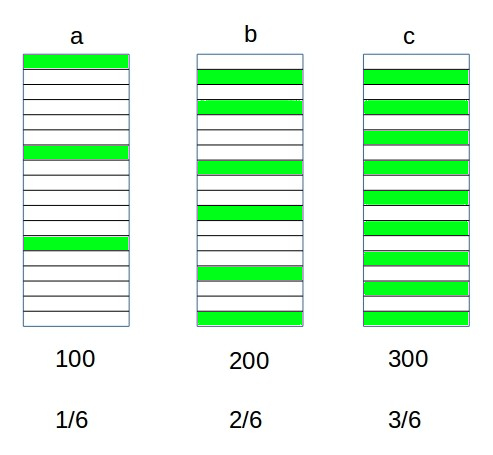
\includegraphics[width=0.5\textwidth]{./imagenes/heuristico/valorSoluciones.jpg}
			\caption{Elección ponderada de candidatos}
			\label{fig: Elección ponderada de candidatos}
		\end{center}
	\end{figure}
	
	\item \textbf{Creación de cola de vuelos extra:} estos vuelos conformarán la cola extra que se añadirá al conjunto de vuelos original, haciendo que éstos tengan mayor posibilidad de ser lanzados antes durante las siguientes \textit{N} iteraciones, tal y como se indica en la fase constructiva:
	
	\item \textbf{Descarte de mala solución} si la mejor de las $N$ soluciones candidatas que se analizan no supera el valor de la mejor solución encontrada hasta el momento, se descarta la cola actual y se reinicia el problema.
	Si se da este caso, indicará que la última cola de candidatos que seleccionamos no ha conseguido mejorar la solución del problema, por tanto podemos descartarla.
\end{enumerate}


\subsection{Parámetros heurístico}
Por tanto el heurístico depende de dos parámetros:
\begin{itemize}
	\item \textbf{$N$}: cada cuantas iteraciones actualizamos la cola de vuelos adicional.
	\item \textbf{$G$}: el tamaño máximo de la cola de vuelos adicionales.
\end{itemize}
Tras realizar pruebas sobre distintos problemas, se ha obtenido que las mejores soluciones se tienen a alcanzar con un parámetro $N$ pequeño y $G$ grande, de forma que la cola de vuelos candidatos sea lo más grande posible y que la fase constructiva se realice con mucha frecuencia. Los resultados se pueden observar en la siguiente sección.

\begin{figure}[H]
	\begin{center}
		\centering
		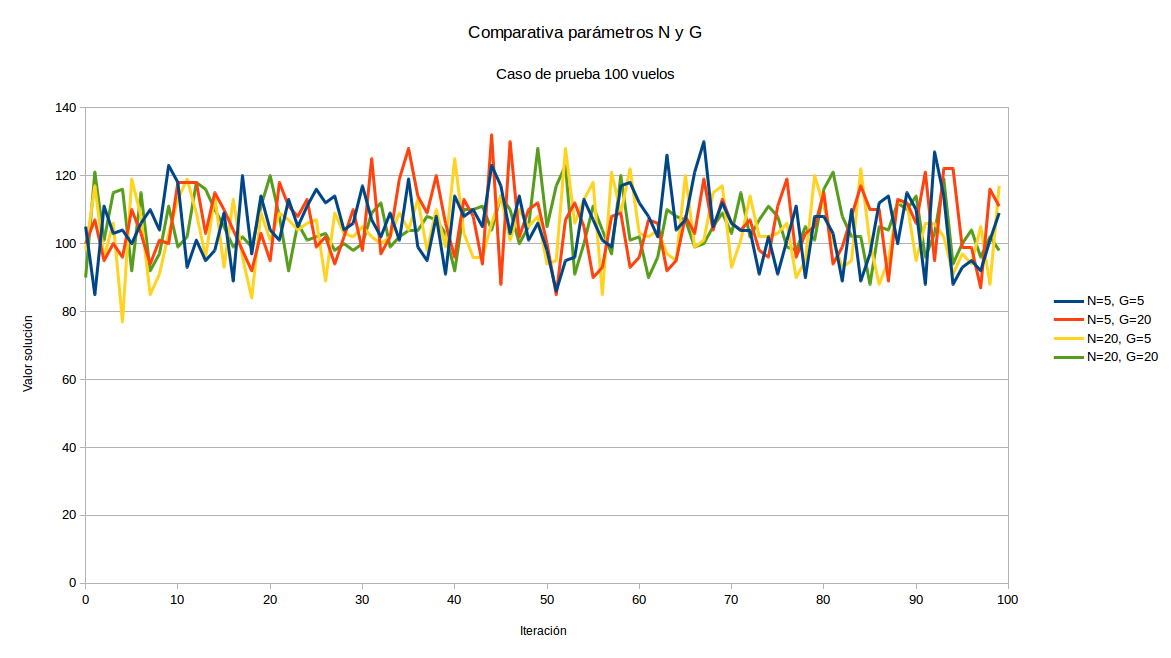
\includegraphics[width=1\textwidth]{./imagenes/heuristico/comparativa_parametros_100_vuelos.png}
		\caption{Comparativa de parámetros G y N}
		\label{fig: Comparativa de parámetros G y N}
	\end{center}
\end{figure}

De esta forma, un alto parámetro $G$ permitirá que muy probablemente muchos de los vuelos que en la mejor solución encontrada hasta ese momento fueron colocados con éxito, se lance, intentando así "reproducir" la mejor solución que se había encontrado. \\
Por contra un bajo parámetro $N$ hará que se cree cada pocas iteraciones una nueva cola de vuelos candidatos, lo que permitirá que en caso de no encontrase rápidamente una solución mejor, se elimine la cola actual y se reinicie el problema.\\
A continuación se muestran los datos obtenidos en una de las simulaciones:



\begin{table}[]
	\centering
	\caption{Comparativa de parámetros $G$ y $N$. Ejemplo problema con 100 vuelos}
	\label{fig: comparativa de parámetros $G$ y $N$. Ejemplo problema con 100 vuelos}
	\begin{tabular}{lllllllllllll}
		& N=2, G=10                                                             & N=2, G=30 & N=2, G=30 &  &  &  &  &  &  &  &  &  \\
		Problema 1 & \multicolumn{1}{c}{\begin{tabular}[c]{@{}c@{}}a\\ b\\ c\end{tabular}} &           &           &  &  &  &  &  &  &  &  &  \\
		Problema 2 &                                                                       &           &           &  &  &  &  &  &  &  &  &  \\
		Problema 3 &                                                                       &           &           &  &  &  &  &  &  &  &  & 
	\end{tabular}
\end{table}


\begin{table}[]
	\centering
	\caption{My caption}
	\label{my-label}
	\begin{tabular}{lllllllllllll}
		\hline
		& N=2, G=10                                                                             & N=2, G=30 & N=2, G=50 & N=5, G=10 & N=5, G=30 & N=5, G=50 & N=10, G=10 & N=10, G=30 & N=10, G=50 & N=20, G=10 & N=20, G=30 & N=20, G=50 \\ \hline
	
		Problema 1 & \multicolumn{1}{c}{\begin{tabular}[c]{@{}c@{}}Máx: 1\\ Med: 2\\ Desv: 3\end{tabular}} &           &           &           &           &           &            &            &            &            &            &            \\
	
		Problema 2 &                                                                                       &           &           &           &           &           &            &            &            &            &            &            \\
		
		Problema 3 &                                                                                       &           &           &           &           &           &            &            &            &            &            &            \\ \hline
	\end{tabular}
\end{table}
Como se puede comprobar, esta combinación de parámetros es la que aporta más aleatoriedad en los resultados, pero es también de media la que aporta mejores resultados, lo que indica que se las malas soluciones son descartadas rápidamente pero se permite explorar un máximo local.

